

\section{Sensitivity of Internally Generated Field to Permeability of the Shield $B_0(\mu)$\label{sec:calculation}}

The presence of a coil inside the innermost passive shield turns the
shield into a return yoke, and generally results in an incease in the
magnitude of $B_0$.  The ratio of this field inside the coil in the
presence of the magnetic shield to that of the coil in free space is
referred to as the reaction factor $C$, and can be calculated
analytically for spherical and infinite cylindrical
geometries~\cite{bib:bidinostimartin,bib:urankar}.  The key issue of
interest for this work is the dependence of the reaction factor on the
permeability $\mu$ of the innermost shield.  Although this dependence
can be rather weak, the constraints on $B_0$ stability are very
stringent.  As a result, even a small change in the magnetic
properties of the innermost shield can result in an unacceptably large
change in $B_0$.


To illustrate, we consider here the model of a sine-theta surface
current on a sphere of radius $a$, inside a spherical shell of inner
radius $R$, thickness $t$, and linear permeability $\mu$.  The uniform
internal field generated by this ideal spherical coil is augmented by
a factor $C$ in the presence of the shield, but is otherwise left
undistorted.  The general reaction factor for this model is given by
Eq.~(38) in Ref.~\cite{bib:bidinostimartin}.  In the high-$\mu$ limit,
with $t\ll R$, the reaction factor can be approximated as
\begin{equation}
C 
 \simeq 1+ \frac{1}{2}\, \left( \frac{a}{R} \right)^{3} \left( 1- \frac{3}{2} \, \frac{R}{t} \, \frac{\muo}{\mu} \right) \, ,
 \label{Csphere}
\end{equation}
which highlights the dependence of $B_0$ on the relative permeability
$\mu_r=\mu/\muo$ of the shield.

Fig.~\ref{fig:Magnetic_Field} shows plots of $B_0$ versus $\mu_r$ for
coil and shield dimensions similar to the ILL nEDM
experiment~\cite{bib:baker,bib:knecht}: $a=0.53$~m, $R= 0.57$~m, and
$t=1.5$~mm.  In addition to analytic calculations, we also include the
results of two axially symmetric simulations conducted using
FEMM~\cite{bib:femm} to assess the effects of geometry and
discretization of the surface current.

%The dashed curve represents the
%results of an analytical calculation for a perfect spherical surface
%current.  For this calculation, a coil of radius 0.53~m inside a
%magnetic shield with inner radius $0.57$~m and thickness 1.5~mm were
%used.  The dimensions have been selected to be comparable to the
%dimensions of the ILL nEDM experiment
%geometry~\cite{bib:baker,bib:knecht}.

\begin{figure}[h!]
\begin{center}
   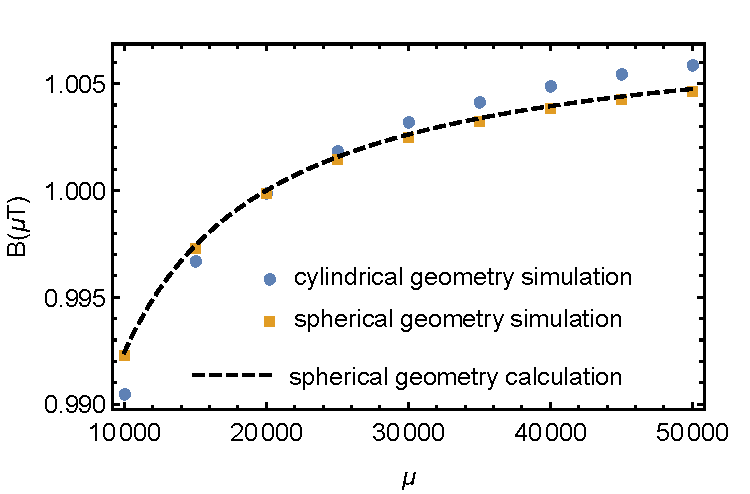
\includegraphics[width=0.7\textwidth]{femm_and_calcs.pdf}
    \caption{Magnetic field at the coil isocenter as a function of
      shield permeability for a geometry similar to the ILL nEDM
      experiment as discussed in the text.  The solid curve is the
      exact calculation for the ideal spherical coil and shield from
      Ref.~\cite{bib:bidinostimartin}; the dashed curve is the
      approximation of Eq.~\ref{Csphere}. The circles and squares are
      the FEMM-based simulations for the spherical and solenoidal
      geometries with discrete currents.  In all cases, current
      magnitudes were chosen to give $B_0=1~\mu$T at $\mu_r=20,000$.}
    \label{fig:Magnetic_Field}
    \end{center}
\end{figure} 


In the first simulation, the same spherical geometry was used as for
the analytical calculations.  However, the surface current was
discretized to 50 individual current loops, inscribed onto a sphere,
and equally spaced vertically (i.e.~a discrete sine-theta coil).  A
square wire profile of side length 1~mm was used.  As shown in
Fig.~\ref{fig:Magnetic_Field}, this simulation gave good agreement
with the analytical calculation.  In the second simulation, a solenoid
coil and cylindrical shield (length/radius~=~2) were used with the
same dimensions as above.  Similarly, the coil was modelled as 50
evenly spaced current loops, with the distance from an end loop to the
inner face of the shield end-cap being half the inter-loop spacing.
In the limit of tight-packing (i.e., a continuous surface current) and
infinite $\mu$, the image currents in the end caps of the shield act
as an infinite series of current loops, giving the ideal uniform field
of an infinitely long solenoid~\cite{bib:lambert,bib:sumner}.  As
shown in Fig.~\ref{fig:Magnetic_Field}, the result is similar to the
spherical case, though the slope of $B_0(\mu_r)$ is somewhat steeper.

In ancillary measurements of shielding factors (discussed briefly in
Section~\ref{sec:previousmeasurement}), we found $\mu_r=20,000$ to
offer a reasonable description of the quasistatic shielding factor. By
evaluating the slope of the analytic curve in
Fig.~\ref{fig:Magnetic_Field} at $\mu_r=20,000$, we estimate that the
scale of the sensitivity of a generic nEDM experiment to global
changes in the magnetic permeability is
$\frac{\mu}{B_0}\frac{dB_0}{d\mu} \sim \frac{3 a^3 }{4R^2 t}
\frac{1}{\mu_r} \sim 0.01$.

For a high-$\mu$ innermost shield, the magnetic field lines emanating
from the coil all return through the shield.  This principle can be
used to estimate the magnetic field internal to the material $B_m$,
and in our studies gave good agreement with FEA-based simulations.
For the solenoidal geometry previously described and used for the
calculations in Fig.~\ref{fig:Magnetic_Field}, $B_m$ is largest in the
side walls of the solenoidal flux return, attaining a maximum value of
170~$\mu$T.  If we assume $\mu_r$=20,000, the $H_m$ field is
0.007~A/m.  Typically the shield is degaussed (idealized) with the
internal coil energized.  After degaussing, $B_m$ must be
approximately the same, since essentially all flux returns through the
shield.  However, the $H_m$ field must become significantly smaller,
as the material must reside on the ideal magnetization curve in
$B_m-H_m$ space.  (For a discussion of the ideal magnetization curve,
we refer the reader to Ref.~\cite{bib:bozorth}.)  In principle, the
$H_m$ field could be reduced by an order of magnitude or more,
depending on the steepness of the ideal magnetization curve near the
origin.  Thus $B_m=170~\mu$T and $H_m<0.007$~A/m set a scale for the
relevant values for nEDM experiments.  Furthermore, the field in the
nEDM measurement volume, as well as in the magnetic shield, must be
stable for periods of typically hundreds of seconds (corresponding to
frequencies $<0.01$~Hz).  This sets the relevant timescale for
magnetic properties most relevant to nEDM experiments.
